\subsection{Beslutningsproblemer og stand-in sprog}
\subsection{P, NP, NPC}
\subsection{Reduktioner}
\subsection{3SAT $\le$ TRIPARTITE MATCHING}
For this reduction we use a combined choice- and consistency gadget. We create one for each variable $x_i$. Each one of such gadget will have k boys, k girls and 2k homes. Where k is equal to the highest occurrence of $x_i$ or $\lnot x_i$.
The uneven numbered homes represent occurrences of x, and the other of $\lnot x$. The boys and girls of these gadgets are only paired with the homes of the same gadget. If a matching exists then $b_i$ is matched with either $g_i$ and $h_{2i}$, or to $g_{i-1}$ and $h_{2i-1}$. The first matching is taken to mean that x = 1 and the second that x = 0.
\\\\
For each clause we add another pair of boy and girl. These will be paired with the corresponding literals in the gadgets. The idea is that if one of these three homes was left unoccupied when the variables were assigned truth values, this means that it corresponds to a true literal, and therefore the clause is satisfied. \textbf{If all three literals in c are false, then the corresponding b/g pair cannot be matched with a home.} \\\\
There are always L extra homes in this construction, and to make sure they can be matched, we introduce L more boy/girl pairs. These pairs all paired with every home in the construction. So these L boy/girl pairs are "easy to please" and are just used to pair the leftover homes. \\\\

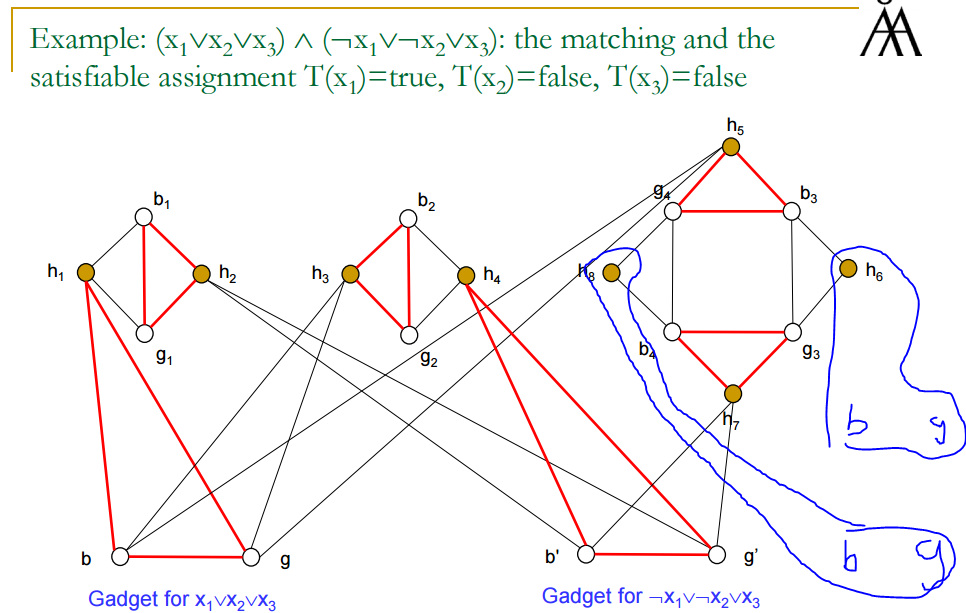
\includegraphics[scale=0.5]{tripartite}
\\
\textbf{Polynomial:} For each variable we make a gadget with at most m boys/girls and 2m homes. For each clause we make a b/g pair. And for each extra home another b/g pair. So it is polynomial.
\\\\
$\implies:$ \\ TODO
\\\\ 
$\impliedby:$ \\ TODO

\newpage
\subsection{Corollary: EXACT COVER BY 3-SETS, SET COVERING AND SET PACKING ARE NP COMPLETE}
TRIPARTITE MATCHING is a special case of EXACT COVER BY 3-SETS. And EXACT COVER BY 3-SETS is a special case of both SET COVER and SET PACKING.\\\\ (https://people.eecs.berkeley.edu/~vazirani/algorithms/chap8.pdf)
\subsubsection{TRIPARTITE MATCHING $\le$ EXACT COVER BY 3-SETS}
Given a TRIPARTITE MATCHING instance: let the EXCB3-S subsets be the same as in the TRIPARTITE MATCHING instance. The EXCB3-S universe is obtained by the union of B G and H.\\\\
Think of EXCB3-S as kind of the same problem but where you can match 3 Boys, or 2 girls and 1 home etc. 
\subsubsection{EXACT COVER BY 3-SETS $\le$ SET COVERING}
EXACT COVER BY 3-SETS instances are a subset of all SET COVERING instances, so the is easy. Nothing is changed and the Budget B = m from the EXCB3-S instance.

\subsubsection{NODE COVER $\le$ 
SET COVERING}
SET COVER is a generalization of NODE COVER. In our construction the universe is all edges in the NODE COVER instance. The subsets are obtained as follows: For each node in the graph, all adjacent edges form a subset.
\subsubsection{EXACT COVER BY 3-SETS $\le$
SET PACKING}
Set the SET PACKING goal k to be m. Then there is a 3-SET cover of size m iff there is a SET PACKING of size m. (Since the input set is 3m). Rest is unchanged.  
\newpage
\subsection{EXACT COVER BY 3-SETS $\le$ KNAPSACK}
Once again we will prove a problem NP hard by showing that a special case is NP hard. The special case of KNAPSACK where $v_i = w_i$ and goal $K = W$ is called SUBSET SUM. (see definition in first section).\\\\
In our construction we think of the 3-sets as binary vectors in $\{0,1\}^{3m}$. And the i'th bit will be 1 iff the i'th element is contained with this particular 3-set. Therefore in each vector, only 3 ones will appear. The vectors can be thought of as binary integers, and set union now resembles integer addition and the goal is to find vectors which sum up to the all 1's vector. \\\\
But binary addition has a carry, which could break the bi-implication. For example 0011 + 0101 + 0111 = 1111, but the sets $\{3,4\}$,$\{2,4\}$,$\{2,3,4\}$ are not disjoint, and their union is not $\{1,2,3,4\}$.\\
To fix this, we think of the numbers in base n+1 instead of 2. since we have n vectors, there can never be a carry.\\\\
The weight goal of $2^{3m}-1$ completes the reduction.\\\\
$\implies$ :\\ If there is an exact cover by 3-sets, then the bit vectors in our construction corresponding to the exact cover will provide a number equal to the wanted K.\\\\
$\impliedby$ :\\ Since we can include every number once, and there is no carry, then there must be vectors which add up to K, and therefore also an exact cover by 3-sets.
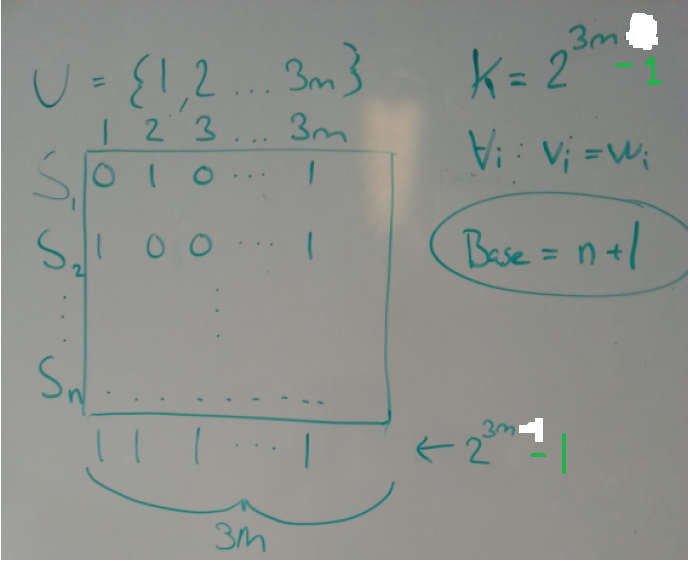
\includegraphics[scale=0.5]{knapsack}
\newpage


